\textit{Cet exercice est un questionnaire à choix multiples. Pour chacune des questions suivantes, une seule des quatre réponses proposées est exacte. Une réponse exacte rapporte un point. Une réponse fausse, une réponse multiple ou l'absence de réponse à une questionne rapporte ni n'enlève de point. Pour répondre, indiquer sur la copie le numéro de la question et la lettre de la réponse choisie. Aucune justification n'est demandée}

\smallskip

\begin{enumerate}
	\item On considère la fonction définie sur $\R$ par $f(x)=x\e^{-2x}$.
	
	On note $f''$ la dérivée seconde de la fonction $f$.
	
	Quel que soit le réel $f$, $f''(x)$ est égal à :
	\begin{enumerate}
		\item $(1-2x)\e^{-2x}$
		\item $4(x-1)\e^{-2x}$
		\item $4\e^{-2x}$
		\item $(x+2)\e^{-2x}$
	\end{enumerate}
	\item Un élève de première générale choisit trois spécialités parmi les douze proposées.
	
	Le nombre de combinaisons possibles est :
	\begin{enumerate}
		\item \num{1728}
		\item \num{1320}
		\item \num{220}
		\item \num{33}
	\end{enumerate}
	\item On donne ci-dessous la représentation graphique de $f'$ fonction dérivée d’une fonction $f$ définie sur $\intervFF{0}{7}$.
	%
	\begin{center}
		\begin{tikzpicture}[x=0.7cm,y=0.7cm,xmin=-1,xmax=8,xgrilles=0.2,ymin=-5,ymax=1,ygrilles=0.2]
			\GrilleTikz \AxesTikz[ElargirOx=0/0,ElargirOy=0/0]
			\AxexTikz[Police=\small]{1,2,...,7} \AxeyTikz[Police=\small]{-4,-3,...,-1} ;
			\draw (-2pt,-2pt) node[below left,font=\small] {0} ;
			\draw[line width=1.25pt,red,samples=250,domain=0:7] plot (\x,{0.05*(\x-2)*(\x-5)*(\x-8)}) ;
		\end{tikzpicture}
	\end{center}
	Le tableau de variation de $f$ sur l’intervalle $\intervFF{0}{7}$ est :
	\begin{multicols}{2}
		\begin{enumerate}
			\item \begin{tikzpicture}[baseline={(T00)},scale=0.95]
				\tkzTabInit[espcl=2]{$x$/0.7,$f$/1.4}{$0$,${3,25}$,$7$}
				\tkzTabVar{-/,+/,-/}
			\end{tikzpicture}
			\item \begin{tikzpicture}[baseline={(T00)},scale=0.95]
				\tkzTabInit[espcl=1.33]{$x$/0.7,$f$/1.4}{$0$,$2$,$5$,$7$}
				\tkzTabVar{+/,-/,+/,-/}
			\end{tikzpicture}
			\item \begin{tikzpicture}[baseline={(T00)},scale=0.95]
				\tkzTabInit[espcl=1.33]{$x$/0.7,$f$/1.4}{$0$,$2$,$5$,$7$}
				\tkzTabVar{-/,+/,-/,+/}
			\end{tikzpicture}
			\item \begin{tikzpicture}[baseline={(T00)},scale=0.95]
				\tkzTabInit[espcl=2]{$x$/0.7,$f$/1.4}{$0$,$2$,$7$}
				\tkzTabVar{-/,+/,-/}
			\end{tikzpicture}
		\end{enumerate}
	\end{multicols}
	\item Une entreprise fabrique des cartes à puces. Chaque puce peut présenter deux
	défauts notés A et B.
	
	Une étude statistique montre que 2,8\,\% des puces ont le défaut A et 2,2\,\% des puces
	ont le défaut B et, heureusement 95,4\,\% des puces n’ont aucun des deux défauts.
	
	La probabilité qu’une puce prélevée au hasard ait les deux défauts est :
	\begin{enumerate}
		\item \num{0,05}
		\item \num{0,004}
		\item \num{0,046}
		\item On ne peut pas le savoir
	\end{enumerate}
	\item On se donne une fonction $f$, supposée dérivable sur $\R$, et on note $f'$ sa fonction
	dérivée.
	
	On donne ci-dessous le tableau de variation de $f$ :
	\begin{center}
		\begin{tikzpicture}
			\tkzTabInit[espcl=2]{$x$/0.7,$f$/1.4}{$-\infty$,$-1$,$+\infty$}
			\tkzTabVar{-/$-\infty$,+/$0$,-/$-\infty$}
		\end{tikzpicture}
	\end{center}
	D’après ce tableau de variation :
	\begin{enumerate}
		\item $f'$ est positive sur $\R$
		\item $f'$ est positive sur $\intervOF{-\infty}{-1}$
		\item $f'$ est négative sur $\R$
		\item $f'$ est positive sur $\intervFO{-1}{+\infty}$
	\end{enumerate}
\end{enumerate}

